\documentclass[a4paper,12pt]{book}


%************
%* packages *
%************


\usepackage[utf8]{inputenc}
\usepackage[italian]{babel}
\usepackage{fancyhdr}
\usepackage{verbatim}
\usepackage{float}
\usepackage{subfigure}
\usepackage[stable]{footmisc}
\usepackage[hang,small,sf]{caption}
\usepackage{cite}
\usepackage{acronym}
\usepackage{sectsty}
\usepackage{listings}
\usepackage[usenames]{color}
\usepackage{graphicx}
\usepackage[italian]{varioref}
\usepackage{lmodern}
\usepackage[left=2.5cm,right=2.5cm,bottom=2.8cm]{geometry}
\usepackage{colortbl}
\usepackage{mathtools}
\usepackage{amsfonts}
\usepackage{imakeidx}\makeindex
% \usepackage[T1]{fontenc}

%*****************
%* nuovi comandi *
%*****************

\newcommand{\abs}[1]{\left|#1\right|}                               % modulo
\newcommand{\dato}{\left|\right.}                                   % probabilit\`{a} condizionata
\newcommand{\fun}[1]{\mathrm{#1}}                                   % stile funzione
\newcommand{\imp}{\;\;\Longrightarrow\;\;}                          % implicazione
\newcommand{\norma}[1]{\left\| #1 \right\|}                         % norma
\newcommand{\prob}[1]{\mathrm{P}\!\left[#1\right]}                  % probabilit\`{a}
\newcommand{\expect}[1]{\mathrm{E}\!\left[#1\right]}                % aspettazione
\newcommand{\sse}{\;\;\Longleftrightarrow\;\;}                      % se e solo se
\newcommand{\vect}[1]{{\boldsymbol{\mathrm{#1}}}}                   % stile vettore
\newcommand{\real}[1]{\fun{Re}\left[#1\right]}                      % parte reale
\newcommand{\imag}[1]{\fun{Im}\left[#1\right]}                      % parte immaginaria
\newcommand{\Dim}[1]{\fun{dim}\left[#1\right]}                      % dimensione di una matrice
\newcommand{\Det}[1]{\fun{det}\left[#1\right]}                      % determinante di una matrice
\newcommand{\Ker}[1]{\fun{ker}\left[#1\right]}                      % ker di una matrice
\newcommand{\rango}[1]{\fun{rango}\left[#1\right]}                  % rango di una matrice
\newcommand{\scalare}[2]{\left\langle #1, #2 \right\rangle}         % prodotto scalare
\newcommand{\blbrace}{\left  \lbrace}                               % parentesi graffa sinistra grande
\newcommand{\brbrace}{\right \rbrace}                               % parentesi graffa destra grande
\newcommand{\sinc}{\fun{sinc}}                                      % sinc
\newcommand{\rect}{\fun{rect}}                                      % rect
\newcommand{\rcos}{\fun{rcos}}                                      % rcos
\newcommand{\sgn}{\fun{sgn}}                                        % sgn
\newcommand{\N}{\mathbb{N}}                                         % insieme dei numeri naturali
\newcommand{\Z}{\mathbb{Z}}                                         % insieme dei numeri interi
\newcommand{\Q}{\mathbb{Q}}                                         % insieme dei numeri razionali
\newcommand{\R}{\mathbb{R}}                                         % insieme dei numeri reali
\newcommand{\C}{\mathbb{C}}                                         % insieme dei numeri complessi
\newcommand{\seq}[2][n]{#2_{0}, #2_{1}, \ldots, \, #2_{#1}}         % sequenza
\newcommand{\Span}[2][n]
{\fun{span} \blbrace #2_{1}, #2_{2}, \ldots, \, #2_{#1} \brbrace}   % spazio generato
\newcommand{\ddt}{\frac{\fun{d}}{\fun{dt}}}                         % derivata
\newcommand{\Div}[2]{#1 \; \mid \; #2}                              % divide
\newcommand{\MCD}[2]{\fun{MCD}\(#1, #2\)}                           % massimo comun divisore
\newcommand{\mcm}[2]{\fun{mcm}\(#1, #2\)}                           % minimo comune multiplo
\newcommand{\goodgap}{
                      \hspace{\subfigtopskip}
                      \hspace{\subfigbottomskip}
                     }                                              % interlinea opportuna per le sottofigure
\newcommand{\eng}[1]{\emph{#1}}                                   % inglese
\newcommand{\virg}[1]{``#1"}                                        % fa una citazione tra virgolette
%\newcommand{\unit}[2]($\frac{\text{#1}}{\text{#2}}$)                % unit\`{a} di misura
\newcommand{\textttvar}[1]{{\ttvar #1}}

\definecolor{gray}{gray}{0.9}
\newcommand{\listato}[1]{\lstset{language=#1, numbers=left, numberstyle=\tiny, stepnumber=2, numbersep=5pt, numberblanklines=false, xleftmargin=5pt, captionpos=b, stringstyle=\ttfamily, columns=flexible, showstringspaces=false, tabsize=2, frame=single, framerule=0pt, backgroundcolor=\color{gray}, basicstyle=\small}}

%****************************
%* ridefinizioni di comandi *
%****************************

\renewcommand{\(}{\left(}                                     % parentesi tonda sinistra grande
\renewcommand{\)}{\right)}                                    % parentesi tonda destra grande
\renewcommand{\[}{\left[}                                     % parentesi quadra sinistra grande
\renewcommand{\]}{\right]}                                    % parentesi quadra destra grande
\renewcommand{\exp}[1]{\fun{e}^{#1}}                          % esponenziale
\renewcommand{\gcd}[2]{\fun{gcd}\(#1, #2\)}                   % massimo comun divisore

\renewcommand{\lstlistingname}{Codice}
\renewcommand{\lstlistlistingname}{Elenco dei listati codice}
\usepackage{graphicx}
\usepackage{mathtools}
\usepackage[T1]{fontenc}
\usepackage[utf8]{inputenc}
\usepackage[italian]{babel}

\setlength{\parindent}{10pt}



\begin{document}

\begin{titlepage}
\begin{center}
% Upper part of the page. The '~' is needed because \\
% only works if a paragraph has started.

\includegraphics[scale=0.08]{logo.png}\\[1.5cm]
\textsc{\LARGE Universit\`{a} degli Studi di Padova}\\[1.2cm]
\textsc{\Large Dipartimento di Ingegneria dell'Informazione}\\[0.8cm]
\textsc{\Large Corso di Laurea Triennale in}\\[0.5cm]
\textsc{\Large Ingegneria Informatica}\\[2cm]
% Title
{ \LARGE \bfseries Progettazione e realizzazione di un'applicazione Web per la gestione degli eventi di un Conservatorio}\\[2cm]
\textsc{\large Relatore: Prof. Giorgio Maria Di Nunzio}\\[0.5cm]
\textsc{\large Laureando: Davide Marchiori}\\
\vfill
% Bottom of the page
{\large Anno Accademico 2012/2013}
\end{center}
\end{titlepage}


\thispagestyle{empty} % pagina bianca dopo il titolo
\cleardoublepage


\pagenumbering{roman} % numerazione romana per gli indici
\thispagestyle{empty}

\clearpage{\pagestyle{plain}\cleardoublepage}
\tableofcontents

\clearpage{\pagestyle{plain}\cleardoublepage}
\listoffigures

\clearpage{\pagestyle{plain}\cleardoublepage}
\lstlistoflistings


\clearpage{\pagestyle{plain}\cleardoublepage} % numerazione arabica per i capitoli
\pagenumbering{arabic}

%\clearpage{\pagestyle{plain}\cleardoublepage}
%\chapter*{Sommario}
%\addcontentsline{toc}{chapter}{Sommario}
%\newpage
\title{Sommario}
Sono un sommario.



\clearpage{\pagestyle{plain}\cleardoublepage}
%\chapter{Introduzione}
%\newpage
\section{Introduzione}
\subsection{Limiti del computer}
ciao
$$ \epsilon = V * I $$

\includegraphics[scale=0.5]{Immagini/icon.png}


%\clearpage{\pagestyle{plain}\cleardoublepage}
%\chapter{Descrizione del progetto}
%\label{cha:descrizione}
%\input{descrizione.tex}

%\clearpage{\pagestyle{plain}\cleardoublepage}
%\chapter{Progettazione e realizzazione del Database}
%\label{cha:progettazione_concettuale}
%\input{progettazione_concettuale.tex}



%\clearpage{\pagestyle{plain}\cleardoublepage}
%\chapter{Analisi del Framework e software utilizzato}
%\label{cha:analisi_framework}
%\input{analisi_framework.tex}

%\clearpage{\pagestyle{plain}\cleardoublepage}
%\chapter{Conclusioni}
%\label{cha:conclusioni}
%\lvli{Confronto tra D-Wave e computer classico}

\lvlii{Definizione di quantum speedup}
L'interesse nei quantum computer è legato alla loro capacità di essere molto più veloci dei computer tradizionali a risolvere un determinato tipo di problemi, questa capacità prende il nome di \idx{quantum speedup}; a livello matematico è possibile definirlo\cite{DDQS} come il limite del rapporto
$$S = \lim_{N \to \infty} \frac{C(N)}{Q(N)}$$
tra il tempo $C(N)$ necessario per un computer classico a risolvere un problema di dimensioni $N$ e $Q(N)$ il tempo per un computer quantistico per risolvere lo stesso problema. Questa definizione non richiede la capacità di un quantum computer di ridurre un problema da esponenziale a polinomiale (\idx{speedup esponenziale}) come anticipato nell'introduziome ma valuta solo la capacità di \textit{scaling} con l'aumentare delle dimensioni della complessità (\idx{speedup polinomiale}).
Per il calcolo di $Q(N)$ sono state fatte delle simulazioni modificando vari parametri nel D-Wave One e nel D-Wave Two e i loro tempi sono stati valutati come $T_{DW}(N) = Q(N)$. Per quanto riguarda i computer classici sono state eseguite delle simulazioni per ogni $C(N)$ le cui prestazioni sono state misurate compensando la componente parallela fisica\cite{EQA} come $\frac{T_{SA-SQA}(N)}{N} \simeq C(N)$.
Da qui è stata definita\cite{DDQS} la relazione:
$$S_{DW} = \lim_{N \to \infty} \frac{T_{SA-SQA}(N)}{N \cdot T_{DW}(N)}$$


\lvlii{Simulazione del computer quantistico attraverso algoritmi classici}
\cite{EQA}Per analizzare il quantum speedup del D-Wave è stato scelto di confrontarlo con due algoritmi classici molto simili SA e SQA, nella ricerca del ground state attraverso un modello di Ising a due dimensioni dello spin glass.
Questa scelta è dipesa dalla capacità di essere rimappato in un qualsiasi altro problema np-hard.

\begin{figure}[htbp]
  \centering
  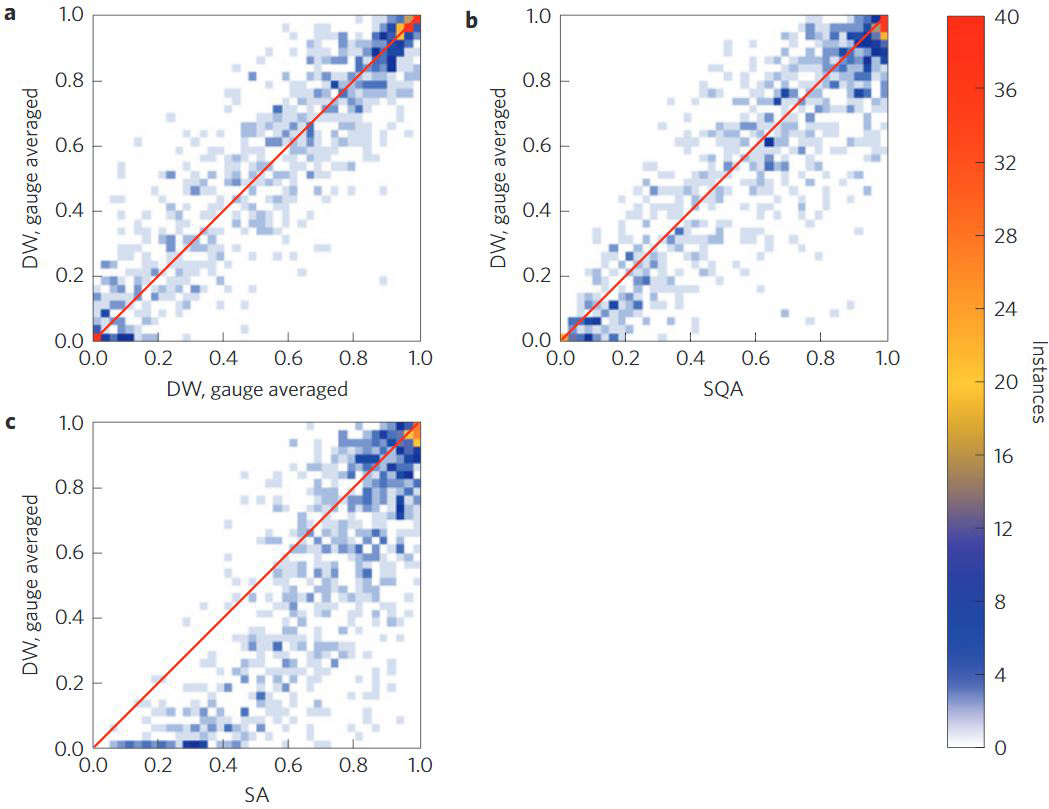
\includegraphics[scale=0.5]{Immagini/correlazione-2-dw.jpg}
  \caption{Correlazione delle prestazione del DW con gli algoritmi classici.}
  \label{figura:correlazione-2-dw}
\end{figure}

I primi esperimenti di comparazione sono stati svolti tramite dei test sulla probabilità di successo $P_{GS}(s) = \frac{M_{GS}}{M}$ nel trovare il ground state. Per ogni dimensione da $N=8$ a $N=108$ sono stati generati $Q=1000$ problemi casuali, e per ogni problema sono state eseguite $M=1000$ istanze di test; i risulati sono stati riportati nella figura \ref{figura:correlazione-2-dw}.
Nel primo grafico (a) è raffigurata la differenza di probabilità di successo tra due configurazioni di parametri impostate sulla stessa macchina della DW per eseguire gli stessi problemi. Nel secondo grafico (b) viene confrontata la macchina DW con il SQA mentre nel terzo (c) sempre la macchina DW ma con il SA. Quello che viene messo in mostra è che il comportamento della macchina DW è molto più simile al SQA che al SA deducibile dalla presenza di una distribuzione bimodale, visibile all'estremità della linea rossa rappresentante la perfetta correlazione, sia per il DW che per il SQA ma non presente nel SA.
I $\chi^2$-test hanno sottolineato quello già visibile fornendo i seguenti valori di comparazione $\chi_{DW}^2(s) \approx 1 \cdot M$, $\chi_{SQA}^2(s) \approx 1,25 \cdot M$, $\chi_{SA}^2(s) \geq 2.24 \cdot M$ con:
$$\chi^2(s) = \sum_{i=0}^I \frac{(P_{GS2}(s, i) -P_{GS1}(s, i))^2}{P_{GS1}(s, i)}$$

Ulteriori test sono stati fatti per capire il legame tra SQA e DW. Nel DW sono stati svolti delle prove che hanno confermato che il comportamento bimodale aumenta con il diminuire della temperatura, ovvero con l'aumentare dell'effetto quantistico rispetto a quello termico. Per il SQA sono stati svolte ulteriori analisi sullo studio della distanza tra il ground state e il primo stato di eccitazione $\Delta E = E_{1} - E_{GS}$ svolgendo in dettaglio due tipologie di problemi o semplici o complessi. È stato ricavato che sia nei problemi semplici che in quelli complessi ci sono due punti critici dove $\Delta E \to 0$, nel punto di inversione di simmetria e per $A/B \to 0$, nessuno di questi influisce nel calcolo. Nei problemi complessi è stato individuato un punto critico aggiuntivo per $A/B \approx 0.5$ che può causare il fallimento dell'annealing dato a differenza delle altre due si trova nella parte centrale del calcolo come è mostatro in figura \ref{figura:ground-state-gap}.

\begin{figure}[htbp]
  \centering
  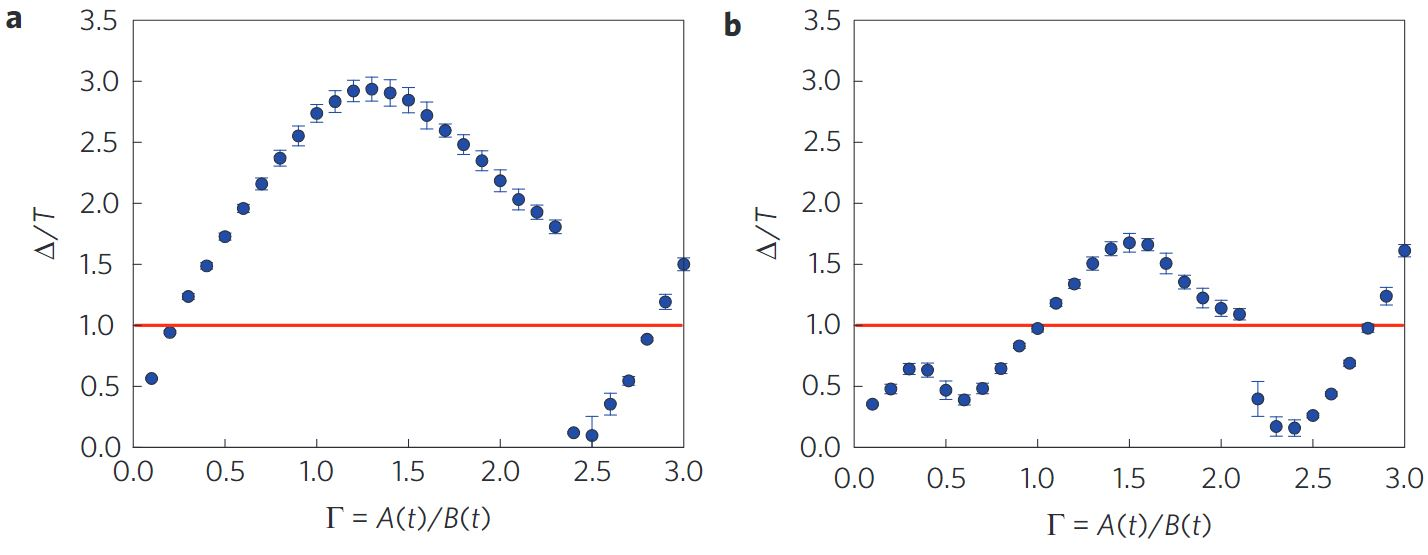
\includegraphics[scale=0.38]{Immagini/ground-state-gap.jpg}
  \caption{$\Delta E$ per un problema semplice (\textbf{a}) e per uno complesso (\textbf{b}).}
  \label{figura:ground-state-gap}
\end{figure}

Un'altra osservazione derivante dallo studio dei $\Delta E$ è che problemi semplici presentano distanze di Hamming piccole tra il risultato dell'algoritmo e il ground state più vicino, mentre problemi complessi hanno distanze più grandi.

Combinando tutte queste osservazioni si ottiene la conferma della similitudine tra DW e SQA, infatti il SQA divide i problemi in due categorie semplici e complessi. Con i problemi complessi contrariamente al SA il SQA riduce i grossi gap in piccole matrici di tunneling aumentando la probabilità di finire in uno stato di bassa energia.

\lvlii{Mancanza di speedup}
\cite{DDQS}Per determinare lo speedup si è deciso quindi di confrontare il DW sia con SQA(PIMC) che con il SA confrontando i valori medi dei tempi in 1000 istanze per risolvere un problema con probabilità $P_p=0.99$.
Per far ciò si sono eseguiti $R$ ripetizioni per ogni istanza generando un tempo $t_i = R_i(t_a) \cdot t_a$ dove il numero di ripetizioni è stato calcolato per rispettare la probabilità $P_p$ fissando la media geometrica di successo $\bar{s}(t_a)$ attraverso la formula:
$$R(t_a) = \left\lceil\frac{\ln(1 - P_p)}{\ln(1 - \bar{s}(t_a))}\right\rceil$$
Dal lato delle simulazioni si è deciso di contare il numero di MCS e di moltiplicare il valore per il tempo minimo di calcolo $t_a^{SA}, t_a^{SQA}$.
Per quanto riguarda il DW la procedura è stata più complessa perché partendo dal tempo globale bisognava rimuovere il tempo di setup e ricavarsi quindi il tempo di annealing $t_a^{DW}$. Il tempo $t_a^{DW}$ si è rivelato essere molto delicato dato il legame con altri due parametri: $r$ il valore massimo dei parametri di accoppiamento spaziale tra spin e $N$ dimensione del problema. Si è scelto di calcolare il tempo ottimo per un numero limitato di dimensione del problema ($N$) facendo variare $r$, in questo modo il tempo $t_a^{DW}$ che risulta subottimo per $N$ troppo grandi è stato calcolato in modo tale che risultasse accettabile in base ai test eseguiti.

% \cite{DDQS}Sono state fatte delle comparazioni tra SA e DW\cite{DDQS} e tra i vari SQA e DW\cite{QVC}, ognuna delle quali ha dimostrato che il DW dopo un certo numero $N_{crit}$ di spin inizia ad avere prestazioni inferiori rispetto ad entrambi gli algoritmi, e ciò denota un'evidente prova della \idx{mancanza di speedup} ad oggi dei sistemi testati. L'assenza di speedup non vuol dire che l'architettura così pensata non possa presentare speedup in futuro, infatti gli ottimi risultati ottenuti dal DW sotto $N_{crit}$ fanno pensare che il quantum speedup non sia raggiunto a causa della difficile calibrazione e rimozione dei rumori termici per grandi $N$ come spiegato nel capitolo dell'architettura.

\lvlii{Confronto tra algoritmi classici}
Nonostante il fallimento nel dimostrare lo speedup si è scoperto un'altro legame molto interessante, quello tra il SQA e il DW. Tale algoritmo approssima bene il comportamento per $N$ molto piccoli e per $N$ molto grandi\cite{EQA}, in particolare la sua versione continua CT-SQA\cite{QVC}. Infatti confermato dalle basi teoriche, solo il CT-SQA è un vero simulatore per il QA perché le approssimazioni utilizzate per il cambiamento da modello quantistico a classico sono fatte considerando evoluzioni continue del sistema.

Il CT-SQA si è rivelato avere prestazioni molto inferiori rispetto al DT-SQA visto che il calcolo usato per ottenerlo attraverso la media delle energie, introduce un'energia residua. Questa osservazione potrebbe essere anche il sintomo che il QA non riesca mai a raggiungere le prestazioni del DT-SQA per colpa proprio di energie residue dovute alla continuità e non dall'effetto termico.

\begin{figure}[htbp]
  \centering
  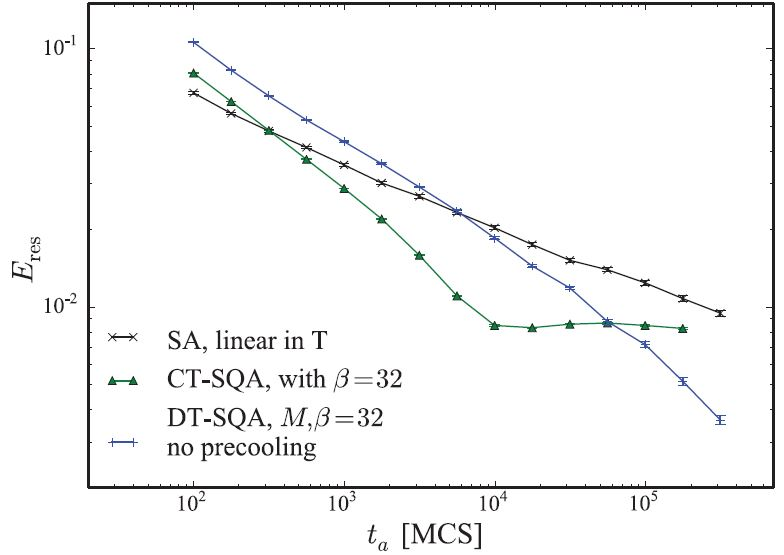
\includegraphics[scale=0.6]{Immagini/residua.jpg}
  \caption{Energie residue nell'esecuzione degli algoritmi.}
  \label{figura:residua}
\end{figure}

\lvlii{Conclusioni}
In conclusione è possibile che in futuro la D-Wave possa ottimizzare il QA in modo tale che presenti uno speed-up rispetto al CT-SQA ma che non sia sufficiente a superare le prestazioni del DT-SQA che si è rivelato essere un ottimo algoritmo per i computer tradizionali. Tutti gli esperimenti realizzati fino ad ora sono stati eseguiti su un modello di Ising a due dimensioni, con condizioni al contorno periodiche, si augura che con il miglioramento dell'architettura del DW sia possibile confrontare modelli a tre dimensioni o superiori e che possano avere risultati differenti.


%\clearpage{\pagestyle{plain}\cleardoublepage}
%\appendix
%\chapter{Codice SQL}
%\label{cha:codice_sql}
%\input{codice_sql.tex}
%%%
%\newpage
\begin{thebibliography}{99}
  \bibitem{mqm} Atkins Friedman, \textit{Meccanica quantistica molecolare}, 1983
  \bibitem{aci} P. I. Bunyk, E. Hoskinson, M. W. Johnson, E. Tolkacheva, F. Altomare, A. J. Berkley, R. Harris, J. P. Hilton, T. Lanting, J. Whittaker, \textit{Architectural considerations in the design of a superconducting quantum annealing processor}, 2014
  \bibitem{qas} M. W. Johnson, M. H. S. Amin, S. Gildert, T. Lanting, F. Hamze, N. Dickson, R. Harris, A. J. Berkley, J. Johansson, P. Bunyk, E. M. Chapple, C. Enderud, J. P. Hilton, K. Karimi, E. Ladizinsky, N. Ladizinsky, T. Oh, I. Perminov, C. Rich, M. C. Thom, E. Tolkacheva, C. J. S. Truncik, S. Uchaikin, J. Wang, B. Wilson, G. Rose, \textit{Quantum annealing with manufactured spins}, 2011
  \bibitem{mcp} E. D. Dahl, \textit{Programming with D-Wave: Map Coloring Problem}, 2013
  \bibitem{jjq} John M. Martinis, Kevin Osborne, \textit{Superconducting Qubits and the Physics of
Josephson Junctions}, 2004
\end{thebibliography}


\end{document}
